\documentclass[11pt,a4paper,oneside]{book}

% ============================================
% PACKAGES
% ============================================
\usepackage[utf8]{inputenc}
\usepackage[T1]{fontenc}
\usepackage[english]{babel}
\usepackage{geometry}
\usepackage{titlesec}
\usepackage{fancyhdr}
\usepackage{graphicx}
\usepackage{xcolor}
\usepackage{tcolorbox}
\usepackage{tikz}
\usepackage{listings}
\usepackage{hyperref}
\usepackage{tabularx}
\usepackage{booktabs}
\usepackage{enumitem}
\usepackage{fontawesome5}
\usepackage{multicol}
\usepackage{menukeys}

% ============================================
% DOCUMENT GEOMETRY
% ============================================
\geometry{
    a4paper,
    left=2.5cm,
    right=2.5cm,
    top=2.5cm,
    bottom=3cm,
    headheight=15pt
}

% ============================================
% COLOR DEFINITIONS
% ============================================
\definecolor{rnblue}{RGB}{97,218,251}
\definecolor{rndark}{RGB}{32,35,42}
\definecolor{nodejsgreen}{RGB}{67,133,61}
\definecolor{primarydark}{RGB}{40,44,52}
\definecolor{codebackground}{RGB}{245,245,250}
\definecolor{stringcolor}{RGB}{0,128,0}
\definecolor{keywordcolor}{RGB}{0,0,255}

% ============================================
% TIKZ LIBRARIES
% ============================================
\usetikzlibrary{shapes,arrows,positioning,shadows,calc}

% ============================================
% HYPERREF SETUP
% ============================================
\hypersetup{
    colorlinks=true,
    linkcolor=primarydark,
    filecolor=rnblue,
    urlcolor=rnblue,
    pdftitle={React Native Simplified Guide},
    pdfauthor={Mausam Kar},
    pdfsubject={Mobile Development},
    pdfkeywords={React Native, JavaScript, Mobile, iOS, Android}
}

% ============================================
% CHAPTER & SECTION STYLING
% ============================================
\titleformat{\chapter}[block]
  {\normalfont\huge\bfseries\color{rndark}}
  {\colorbox{rnblue}{\parbox{1.5cm}{\centering\textcolor{black}{\fontsize{40}{48}\selectfont\thechapter}}}}
  {1em}
  {\Huge}
  [\vspace{2ex}\titlerule]

\titleformat{\section}
  {\normalfont\Large\bfseries\color{rndark}}
  {\thesection}
  {1em}
  {}
  [\vspace{0.5ex}{\color{rnblue}\titlerule[1pt]}]

% ============================================
% BOX STYLES
% ============================================
\tcbuselibrary{skins,breakable}

\newtcolorbox{conceptbox}{
    colback=rnblue!10,
    colframe=rnblue!80!black,
    fonttitle=\bfseries,
    title=Concept,
    boxrule=1pt,
    arc=3pt,
    breakable
}

\newtcolorbox{comparisonbox}{
    colback=orange!10,
    colframe=orange!80!black,
    fonttitle=\bfseries,
    title=React Web vs React Native,
    boxrule=1pt,
    arc=3pt,
    breakable
}

\newtcolorbox{nodebox}{
    colback=nodejsgreen!10,
    colframe=nodejsgreen,
    fonttitle=\bfseries\color{white},
    title=Node.js Connection,
    boxrule=1pt,
    arc=3pt,
    breakable
}

% ============================================
% CODE LISTING STYLE
% ============================================
\lstset{
    backgroundcolor=\color{codebackground},
    basicstyle=\ttfamily\small,
    keywordstyle=\color{keywordcolor}\bfseries,
    stringstyle=\color{stringcolor},
    commentstyle=\color{gray}\itshape,
    numberstyle=\tiny\color{gray},
    numbers=left,
    breaklines=true,
    frame=single,
    rulecolor=\color{lightgray},
    tabsize=2,
    captionpos=b,
    showstringspaces=false
}

% ============================================
% DOCUMENT START
% ============================================
\begin{document}

% ============================================
% TITLE PAGE
% ============================================
\begin{titlepage}
\begin{tikzpicture}[remember picture,overlay]
    \fill[rndark] (current page.south west) rectangle (current page.north east);
    
    % React Logo Circles
    \draw[rnblue, thick] (current page.center) ellipse (3cm and 1cm);
    \draw[rnblue, thick, rotate=60] (current page.center) ellipse (3cm and 1cm);
    \draw[rnblue, thick, rotate=120] (current page.center) ellipse (3cm and 1cm);
    \fill[rnblue] (current page.center) circle (0.5cm);
    
    \node[text width=14cm,align=center] at ([yshift=-2cm]current page.center) {
        {\Huge\bfseries\color{white} REACT NATIVE}\\[0.5cm]
        {\LARGE\color{rnblue} The Simplified Guide}\\[1cm]
        {\large\color{lightgray} Learn Once, Write Anywhere}\\[3cm]
        {\Large\color{white} Cross-Platform Mobile Development}\\[0.3cm]
        {\large\color{lightgray} JavaScript • React • iOS • Android}\\[4cm]
        {\LARGE\bfseries\color{white} Mausam Kar}\\[0.3cm]
    };
\end{tikzpicture}
\end{titlepage}

\frontmatter
\tableofcontents

\mainmatter

% ============================================
% CHAPTER 1: WHAT IS IT?
% ============================================
\chapter{What is React Native?}

\section{Introduction}

\begin{conceptbox}
\textbf{React Native} is a framework that allows you to build real, native mobile applications for iOS and Android using \textbf{JavaScript} and \textbf{React}.
\end{conceptbox}

Instead of writing swift/Obj-C for iOS and Java/Kotlin for Android, you write JavaScript code that renders native views on both platforms. It is \textbf{NOT} a "webview" app (like a website running in an app shell); it renders real native UI components.

\section{Why is it popular?}

\begin{enumerate}
    \item \textbf{Cross-Platform}: Write one codebase, run on iOS and Android. Saves massive time and money.
    \item \textbf{Native Performance}: Uses native components, so it feels smooth and fast.
    \item \textbf{Developer Experience}: Features like "Fast Refresh" let you see code changes instantly without rebuilding.
    \item \textbf{Community}: Huge ecosystem of libraries and tools.
\end{enumerate}

% ============================================
% CHAPTER 2: REACT VS REACT NATIVE
% ============================================
\chapter{React Web vs React Native}

\section{Similarities & Differences}

If you know React for the web, you already know 80\% of React Native. The logic is the same (components, props, state, hooks); only the \textit{rendering} is different.

\begin{comparisonbox}
\begin{tabularx}{\textwidth}{X | X}
\textbf{React (Web)} & \textbf{React Native (Mobile)} \\
\midrule
Uses HTML Tags: \texttt{<div>}, \texttt{<span>}, \texttt{<p>} & Uses Native Components: \texttt{<View>}, \texttt{<Text>} \\
\midrule
Styling: CSS files, className & Styling: JavaScript Objects (\texttt{StyleSheet}) \\
\midrule
Navigation: URL based (React Router) & Navigation: Screen based (React Navigation) \\
\midrule
Platform: Browser DOM & Platform: Mobile UI APIs \\
\end{tabularx}
\end{comparisonbox}

\section{The Core Replacement}

\begin{itemize}
    \item Instead of \texttt{<div>}, use \textbf{\texttt{<View>}}.
    \item Instead of \texttt{<p>} or \texttt{<h1>}, use \textbf{\texttt{<Text>}}. (Text \textit{must} be inside a \texttt{<Text>} component).
    \item Instead of \texttt{<button>}, use \textbf{\texttt{<Pressable>}} or \textbf{\texttt{<TouchableOpacity>}}.
    \item Instead of \texttt{<img>}, use \textbf{\texttt{<Image>}}.
\end{itemize}

% ============================================
% CHAPTER 3: THE NODE.JS CONNECTION
% ============================================
\chapter{How it Runs \& Node.js}

\section{Role of Node.js}

Beginners often ask: \textit{"Does this run on Node.js?"}

\begin{nodebox}
\textbf{The Answer: Yes and No.}

\begin{itemize}
    \item \textbf{Development (YES):} Your computer uses Node.js to run the \textbf{Metro Bundler}. This tool "bundles" your many JavaScript files into one package that the app can read. It's like a server running on your laptop that talks to your phone.
    \item \textbf{On Device (NO):} The app on the phone does \textit{not} run Node.js. It runs a JavaScript Engine (like Hermes or JavaScriptCore).
\end{itemize}
\end{nodebox}

So, you need Node.js installed on your computer to \textit{build} and \textit{manage} the project (using npm/yarn), but the app itself runs independently on the phone's engine.

\section{Architecture Simplified}

\begin{center}
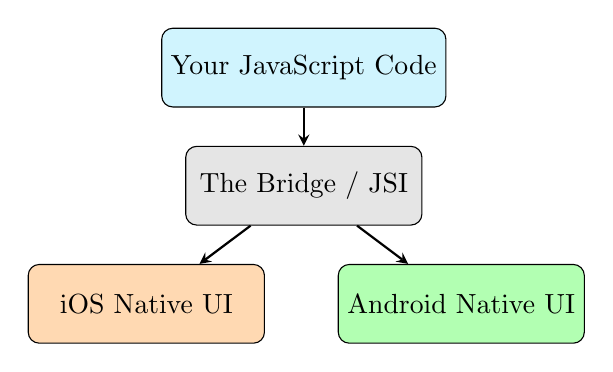
\begin{tikzpicture}[
    node distance=1.5cm,
    box/.style={rectangle, draw=black, rounded corners, minimum width=3cm, minimum height=1cm, text centered},
    arrow/.style={->, >=stealth, thick}
]

\node[box, fill=rnblue!30] (js) {Your JavaScript Code};
\node[box, fill=gray!20, below of=js] (bridge) {The Bridge / JSI};
\node[box, fill=orange!30, below of=bridge, xshift=-2cm] (ios) {iOS Native UI};
\node[box, fill=green!30, below of=bridge, xshift=2cm] (android) {Android Native UI};

\draw[arrow] (js) -- (bridge);
\draw[arrow] (bridge) -- (ios);
\draw[arrow] (bridge) -- (android);

\end{tikzpicture}
\end{center}

1. \textbf{JS Thread}: Runs your logic (calculations, API calls).
2. \textbf{Native Thread}: Renders pixels on the screen.
3. \textbf{Communication}: They talk to each other to update the screen.

% ============================================
% CHAPTER 4: CORE COMPONENTS
% ============================================
\chapter{Core Components & Examples}

\section{Basic Component Structure}

Here is a simple "Hello World" app. Notice how similar it is to React.

\begin{lstlisting}[language=JavaScript, caption=App.js]
import React from 'react';
import { View, Text, StyleSheet } from 'react-native';

const App = () => {
  return (
    // View is like a div container
    <View style={styles.container}>
      <Text style={styles.title}>Hello, React Native!</Text>
      <Text style={styles.subtitle}>My first mobile app.</Text>
    </View>
  );
};

// Styles are written in JS, similar to CSS
const styles = StyleSheet.create({
  container: {
    flex: 1, // Fill the screen
    justifyContent: 'center', // Network center vertically
    alignItems: 'center', // Center horizontally
    backgroundColor: '#f5f5f5',
  },
  title: {
    fontSize: 24,
    fontWeight: 'bold',
    color: '#333',
  },
  subtitle: {
    fontSize: 16,
    color: '#666',
  }
});

export default App;
\end{lstlisting}

\section{Handling User Input}

Using \texttt{TextInput} and \texttt{useState}.

\begin{lstlisting}[language=JavaScript, caption=Input Example]
import React, { useState } from 'react';
import { View, TextInput, Text, Button } from 'react-native';

const InputScreen = () => {
  const [name, setName] = useState('');

  return (
    <View style={{ padding: 20 }}>
      <Text>Enter your name:</Text>
      
      <TextInput
        style={{
            height: 40,
            borderColor: 'gray',
            borderWidth: 1,
            marginBottom: 10,
            padding: 8
        }}
        placeholder="Type here..."
        onChangeText={text => setName(text)}
        value={name}
      />
      
      <Text>Your name is: {name}</Text>
    </View>
  );
};
\end{lstlisting}

\section{Scrolling Lists}

Mobile apps often have long lists. Use \texttt{FlatList} for performance. It only renders items currently visible on screen.

\begin{lstlisting}[language=JavaScript, caption=FlatList Example]
import React from 'react';
import { FlatList, Text, View } from 'react-native';

const data = [
  { id: '1', title: 'Buy Milk' },
  { id: '2', title: 'Walk the dog' },
  { id: '3', title: 'Code React Native' },
];

const TodoList = () => {
  return (
    <FlatList
      data={data}
      keyExtractor={item => item.id}
      renderItem={({ item }) => (
        <View style={{ padding: 10, borderBottomWidth: 1 }}>
          <Text>{item.title}</Text>
        </View>
      )}
    />
  );
};
\end{lstlisting}

% ============================================
% CHAPTER 5: STYLING WITH FLEXBOX
% ============================================
\chapter{Styling (Flexbox)}

\section{Layout Simplified}

React Native uses \textbf{Flexbox} for layout. It works almost exactly like CSS Flexbox, with one major difference:
\begin{center}
\textbf{The default direction is COLUMN (vertical), not ROW.}
\end{center}

\begin{code}
\begin{itemize}
    \item \textbf{flex: 1} Take up all available space.
    \item \textbf{flexDirection: 'row'} Arrange items left-to-right.
    \item \textbf{justifyContent} Align along the main axis (vertical by default).
    \item \textbf{alignItems} Align along the cross axis (horizontal by default).
\end{itemize}
\end{code}

\begin{lstlisting}[language=JavaScript, caption=Layout Example]
<View style={{ flex: 1, flexDirection: 'row' }}>
    <View style={{ width: 50, height: 50, backgroundColor: 'red' }} />
    <View style={{ width: 50, height: 50, backgroundColor: 'blue' }} />
    <View style={{ width: 50, height: 50, backgroundColor: 'green' }} />
</View>
\end{lstlisting}
This creates a row of three colored squares.

% ============================================
% CHAPTER 6: FEATURES
% ============================================
\chapter{Key Features Offered}

\section{1. Fast Refresh}
When you save a file, the app updates almost instantly. It keeps your current data (state), so you don't lose where you are in the app.

\section{2. Native Modules}
If React Native doesn't support a specific phone feature (like a specific Bluetooth sensor), you can write a "Native Module" in Swift or Java and call it from JavaScript.

\section{3. Expo Framework}
A toolchain built \textit{on top} of React Native.
\begin{itemize}
    \item \textbf{Expo Go App}: Run your code on a real phone instantly without setting up Android Studio or Xcode.
    \item \textbf{Over-the-Air Updates}: Fix bugs and push updates to users without waiting for App Store review.
\end{itemize}

% ============================================
% CHAPTER 7: GETTING STARTED
% ============================================
\chapter{How to Start}

\section{The Easiest Way: Expo}

\begin{enumerate}
    \item \textbf{Install Node.js} on your computer.
    \item \textbf{Open Terminal} and run:
    \begin{lstlisting}[language=bash]
    npx create-expo-app my-first-app
    cd my-first-app
    npx expo start
    \end{lstlisting}
    \item \textbf{Download "Expo Go"} on your phone (iOS or Android).
    \item \textbf{Scan the QR code} shown in your terminal.
    \item \textbf{Code!} Edit \texttt{App.js} and see changes instantly.
\end{enumerate}

\begin{tcolorbox}[colback=green!10, colframe=green!70!black, title=Summary]
React Native is the best way for web developers to become mobile developers. You use your existing JavaScript skills to build high-quality, performant, native mobile apps.
\end{tcolorbox}

\end{document}
